%\documentclass[
  bibliography=totoc,     % Literatur im Inhaltsverzeichnis
  captions=tableheading,  % Tabellenüberschriften
  titlepage=firstiscover, % Titelseite ist Deckblatt
]{scrartcl}

% Paket float verbessern
\usepackage{scrhack}

% Warnung, falls nochmal kompiliert werden muss
\usepackage[aux]{rerunfilecheck}

% unverzichtbare Mathe-Befehle
\usepackage{amsmath}
% viele Mathe-Symbole
\usepackage{amssymb}
% Erweiterungen für amsmath
\usepackage{mathtools}

% Fonteinstellungen
\usepackage{fontspec}
% Latin Modern Fonts werden automatisch geladen
% Alternativ zum Beispiel:
%\setromanfont{Libertinus Serif}
%\setsansfont{Libertinus Sans}
%\setmonofont{Libertinus Mono}

% Wenn man andere Schriftarten gesetzt hat,
% sollte man das Seiten-Layout neu berechnen lassen
\recalctypearea{}

% deutsche Spracheinstellungen
\usepackage[ngerman]{babel}


\usepackage[
  math-style=ISO,    % ┐
  bold-style=ISO,    % │
  sans-style=italic, % │ ISO-Standard folgen
  nabla=upright,     % │
  partial=upright,   % │
  mathrm=sym,        % ┘
  warnings-off={           % ┐
    mathtools-colon,       % │ unnötige Warnungen ausschalten
    mathtools-overbracket, % │
  },                       % ┘
]{unicode-math}

% traditionelle Fonts für Mathematik
\setmathfont{Latin Modern Math}
% Alternativ zum Beispiel:
%\setmathfont{Libertinus Math}

\setmathfont{XITS Math}[range={scr, bfscr}]
\setmathfont{XITS Math}[range={cal, bfcal}, StylisticSet=1]

% Zahlen und Einheiten
\usepackage[
  locale=DE,                   % deutsche Einstellungen
  separate-uncertainty=true,   % immer Unsicherheit mit \pm
  per-mode=symbol-or-fraction, % / in inline math, fraction in display math
]{siunitx}

% chemische Formeln
\usepackage[
  version=4,
  math-greek=default, % ┐ mit unicode-math zusammenarbeiten
  text-greek=default, % ┘
]{mhchem}

% richtige Anführungszeichen
\usepackage[autostyle]{csquotes}

% schöne Brüche im Text
\usepackage{xfrac}

% Standardplatzierung für Floats einstellen
\usepackage{float}
\floatplacement{figure}{htbp}
\floatplacement{table}{htbp}

% Floats innerhalb einer Section halten
\usepackage[
  section, % Floats innerhalb der Section halten
  below,   % unterhalb der Section aber auf der selben Seite ist ok
]{placeins}

% Seite drehen für breite Tabellen: landscape Umgebung
\usepackage{pdflscape}

% Captions schöner machen.
\usepackage[
  labelfont=bf,        % Tabelle x: Abbildung y: ist jetzt fett
  font=small,          % Schrift etwas kleiner als Dokument
  width=0.9\textwidth, % maximale Breite einer Caption schmaler
]{caption}
% subfigure, subtable, subref
\usepackage{subcaption}

% Grafiken können eingebunden werden
\usepackage{graphicx}

% schöne Tabellen
\usepackage{tabularray}
\UseTblrLibrary{booktabs, siunitx}

% Verbesserungen am Schriftbild
\usepackage{microtype}

% Literaturverzeichnis
\usepackage[
  backend=biber,
]{biblatex}
% Quellendatenbank
\addbibresource{lit.bib}
\addbibresource{programme.bib}

% Hyperlinks im Dokument
\usepackage[
  german,
  unicode,        % Unicode in PDF-Attributen erlauben
  pdfusetitle,    % Titel, Autoren und Datum als PDF-Attribute
  pdfcreator={},  % ┐ PDF-Attribute säubern
  pdfproducer={}, % ┘
]{hyperref}
% erweiterte Bookmarks im PDF
\usepackage{bookmark}

% Trennung von Wörtern mit Strichen
\usepackage[shortcuts]{extdash}

\author{%
  Vincent Wirsdörfer\\%
  \href{mailto:vincent.wirsdoerfer@udo.edu}{authorA@udo.edu}%
  \and%
  Joris Daus\\%
  \href{mailto:joris.daus@udo.edu}{authorB@udo.edu}%
}
\publishers{TU Dortmund – Fakultät Physik}


%\begin{document}
\section{Diskussion}
\label{sec:Diskussion}

\subsection{Dynamische Viskosität}

Um die Aussagekraft der empirisch ermittelten Werte der kinematischen Viskosität einordnen zu können, werden 
die berechneten Werte mit den theoretischen Werten abgeglichen. Diesen Gegenüberstellungen erfolgt tabellarisch:

\begin{table*}
    \centering
    \sisetup{per-mode=reciprocal}
    \begin{tblr}{
        colspec = {S S[separate-uncertainty=true, table-format=2.2(1)] S},
        row{1} = {guard, mode=math},
        }
        \toprule
        \text{Temperatur} \ T\mathbin{/}\,\unit{\celsius} & \eta_\text{Messung}\mathbin{/}\,\unit{\gram\per\centi\meter\per\second} & \eta_\text{Theorie}\mathbin{/}\,\unit{\gram\per\centi\meter\per\second} \\
        \midrule 
        20 & 1.356\pm0 0.005 & 1.005 \\ 
        26 & 1.199\pm0 0.004 & 0.874 \\
        35 & 1.013\pm0 0.003 & 0.723 \\
        \bottomrule 
    \end{tblr}
\end{table*}

Die größte prozentuale Abweichung der angegebenen Werte beträgt somit ca. $40.11\,\unit{\percent}$. Aufgrund der Tatsache,
dass die Theoriewerte nur zu bestimmten Temperaturen angegeben sind, werden nur bestimmte Werte der gemessenen Viskositäten 
mit den Literaturwerten verglichen. Somit lässt sich schlussfolgern, dass die allgemeine Entwicklung der dynamischen Viskosität
durch die Messwerte bestätigt wird. Nichtsdestotrotz sind wesentliche Abweichungen von den Werten der Literatur festzustellen.
Diese Fehler können jedoch durch ein breites Spektrum an systematischen Unsicherheiten erklärt werden.

\subsection{Systematische Fehler}

Der wahrscheinlich schwerwiegendste Fehler, welcher bei der Messung gemacht wurde, befindet sich bereits in der Vorbereitung des 
Versuchs. Während die Durchmesser der Kugeln mittels einer Schieblehre hinreichend präzise gemessen werden, ist das angegebene 
Gewicht beider Kugeln anzuzweifeln. Dies liegt daran, dass beide Kugeln signifikante Gebrauchsspuren aufweisen, welche das Gewicht 
und auch die Symmetrie der Kugeln stark beeinflussen. Dementsprechend können Absplitterungen an den Kugeln beispielsweise Turbulenzen
in der Strömung verursachen und zu fehlerbehafteten Ergebnissen führen.\\
Eine weitere Fehlerquelle verbirgt sich in der Messung der Fallzeit mittels der Stoppuhr. Auch wenn die Trägheit der Tastenknöpfe durch 
die eines Smartphones ausgetauscht werden, sind menschliche Einflussfaktoren wie zum Beispiel die Reaktionszeit nicht zu vermeiden.\\
Das letzte markante Fehlerpotential befindet sich erneut in der Messung der Fallzeiten. In diesem Fall wird sich jedoch auf die 
optische Komponente der Messung bezogen. Der exakte Zeitpunkt, an welchem die Kugeln die Messstrecken passieren, ist nur schwer zu 
bestimmen. Dies liegt einerseits an den nicht verhinderbaren Parallaxenfehlern und andererseits an den erschwerten Sichtbedingungen.
Damit ist die Brechung des einfallenden Lichts durch das Glas und das destillierte Wasser gemeint. Auch dieser Faktor kann sich 
schlussendlich auf die berechneten Ergebnisse auswirken.

\subsection{Reynoldszahl}

Wie bereits herausgestellt, kann das Auftreten von Wirbeln und Turbulenzen nicht völlig verhindert werden. Dessen ungeachtet 
verweist die Reynoldszahl mit Werten einem Maximalwert von $Re = 13.86 \pm 0.04$ auf eine stabile und laminare Störung, da dieser Wert weit unter dem kritischen 
Bereich um $R_\text{crit}$ liegt. In disem Fall bezeichnet der Maximalwert jene Reynoldszahl, die bei der Verwendung der größten 
Temperatur berechnet wurde, weil die Strömung bei der größten Temperatur am turbulentesten ist. Dementsprechend liegen alle anderen 
Reynoldszahlen mit kleineren Temperaturen unter dem Maximalwert, wodurch diese Werte noch weiter entfernt vom kritischen Wert befinden.

\section{Anhang}

\begin{figure}[H]
    \centering
    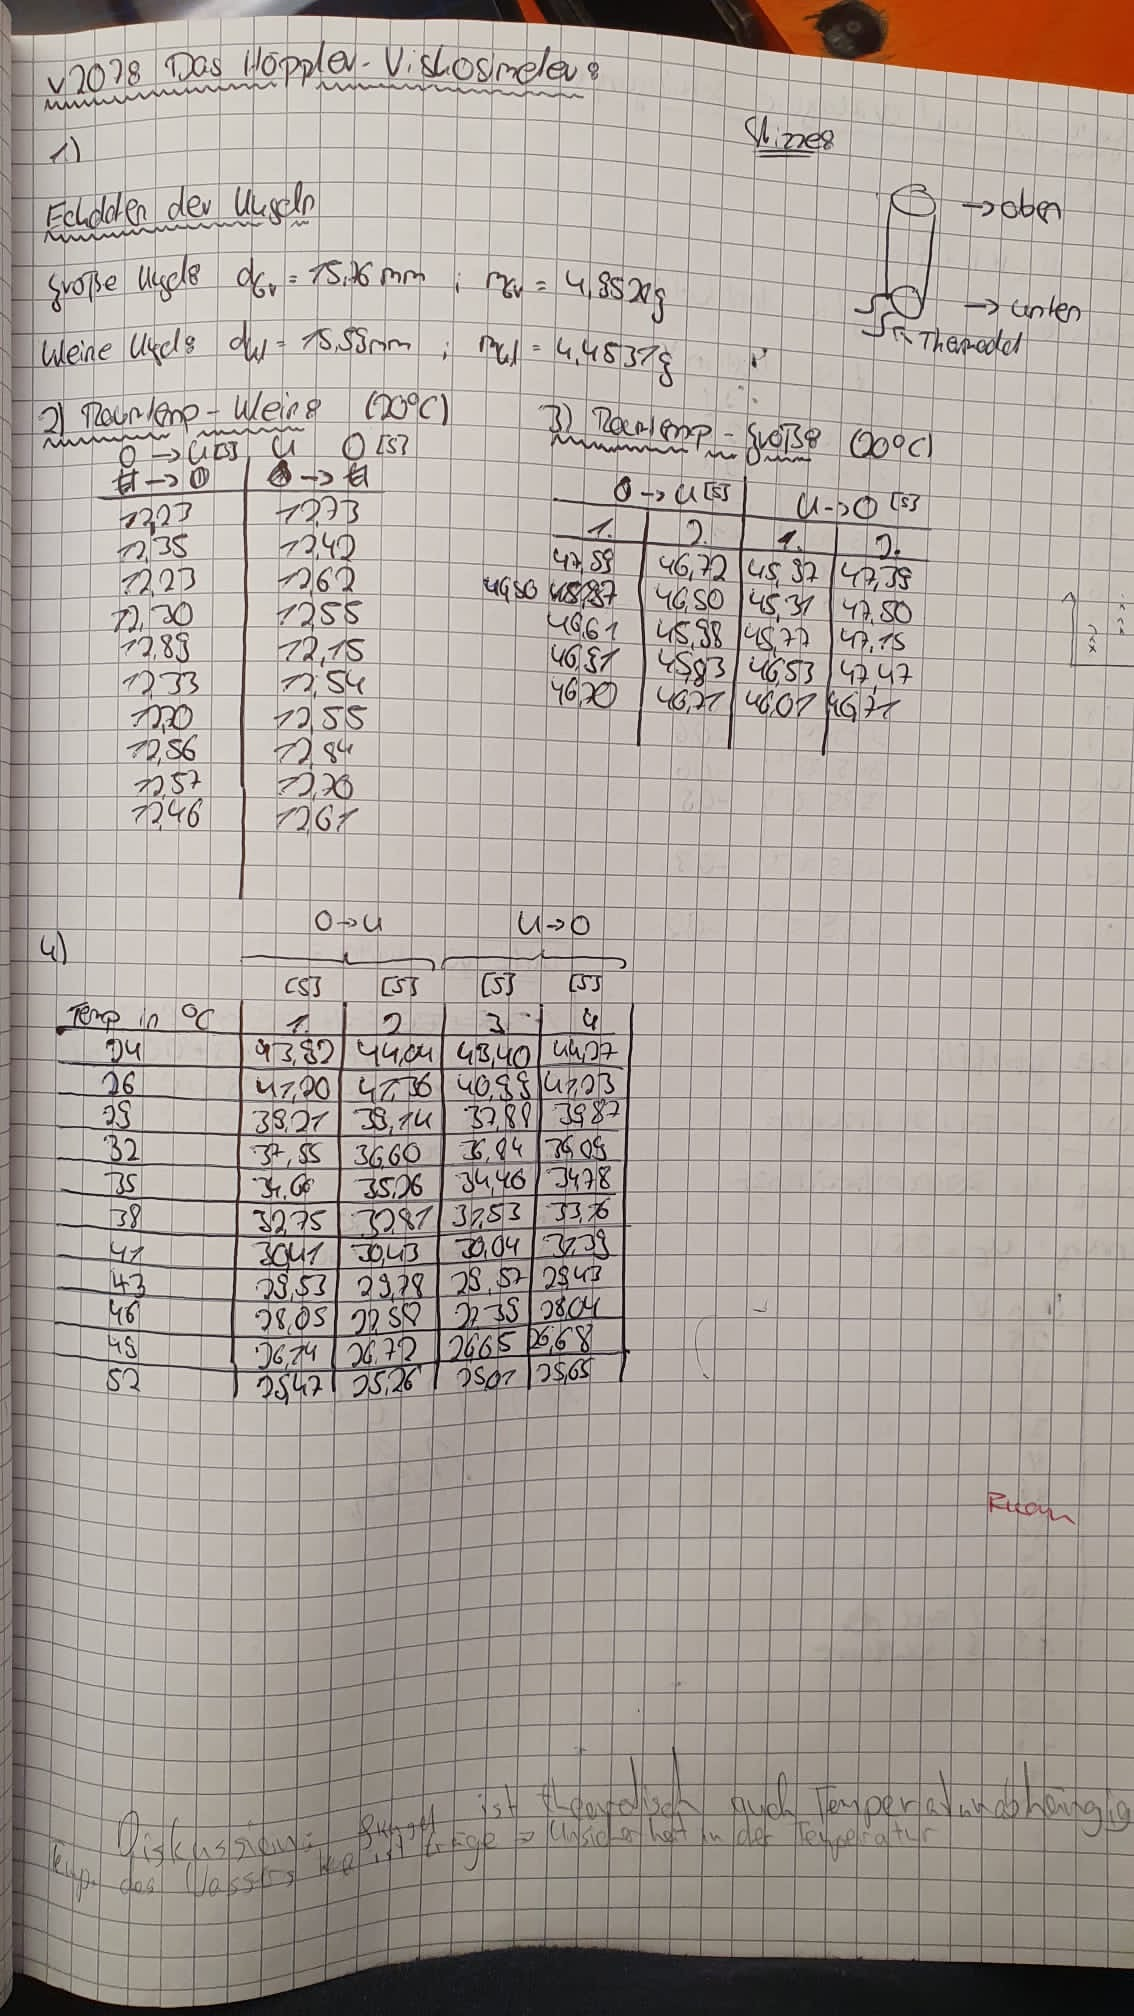
\includegraphics[width=0.7\textwidth]{./content/Originalwerte.JPG}
    \caption{Originalmesswerte des Versuchs v207.}
\end{figure}

%\end{document}
